% Two-column project report, Overleaf-ready.
% The submittable PDF is produced by report/build_report.py (no LaTeX toolchain was
% available locally). This file carries identical content for anyone who prefers to
% compile it; keep the two in step if you edit either.
\documentclass[10pt,twocolumn,a4paper]{article}
\usepackage[margin=14mm]{geometry}
\usepackage{graphicx}
\usepackage{booktabs}
\usepackage{amsmath,amssymb}
\usepackage[colorlinks=true,urlcolor=blue]{hyperref}
\usepackage{microtype}
\setlength{\columnsep}{6mm}
\pagestyle{empty}

\title{\vspace{-8mm}\textbf{Reinforcement Learning for Ambulance Dispatch and
Repositioning}}
\author{Anuj Trivedi (B23CH1006)\\
\small Indian Institute of Technology Jodhpur --- AI Mini Project, Assignment 2\\
\small Repository: \url{https://github.com/anujtrivedi06/ambulance-dispatch-repositioning}}
\date{}

\begin{document}
\twocolumn[{\maketitle}]

\section{Problem and MDP Formulation}
Emergency calls arrive at random locations and times across a city road network. A fleet
of $K$ ambulances must answer them, and an agent makes two coupled decisions:
\textbf{dispatch} (which unit to send to an incoming call) and \textbf{repositioning}
(where each idle unit should wait). The two conflict: sending the nearest unit is optimal
for the call in hand but can strip cover from a dense district, costing the next call more
than it saved this one.

Decisions occur only at irregular event epochs---a call arriving, or a unit becoming
free---so the problem is a \textbf{semi-Markov decision process} rather than a fixed-step
MDP. Transitions carry an elapsed time $\Delta t$, and discounting must respect it.

\section{State Space ($\mathcal{S}$)}
The underlying state is $s = (t, \{(\text{status}_k, \text{loc}_k,
\text{eta}_k)\}_{k=1}^{K}, \text{queue})$: the clock, every unit's status, position and
arrival estimate, and the calls still waiting. With $|V| = 64$ nodes, six unit statuses
and $K = 6$ ambulances, that is on the order of $(64 \times 6)^6 \approx 10^{15}$
configurations before the continuous clock is counted. Exact dynamic programming is
impossible and function approximation is mandatory.

The agent observes an \textbf{11-dimensional post-decision feature vector}: available-unit
fraction; time of day as $(\sin, \cos)$; expected covered demand; worst-zone coverage;
demand-weighted distance to the nearest free unit; four per-zone coverage values; and a
bias term. The post-decision state is a deterministic function of (state, action), so the
agent ranks every candidate action with one forward pass each, with no sampling.

The feature set was cut from twelve after diagnosis on collected data. Three features were
exactly redundant (the design matrix came back rank 9 of 12) and the four per-zone
coverages were collinear at $0.97$ and $1.00$, leaving their weights unidentified. Ridge
regression hid this: value \emph{prediction} stayed accurate because the collinear
directions cancel in-distribution, while the greedy policy degraded, because an action
moves along exactly the direction the data could not identify.

\section{Action Space ($\mathcal{A}$)}
The action space is \textbf{discrete}. At a repositioning epoch the agent chooses one of
$M$ stations, $|\mathcal{A}| = M$ ($M = 4$ in the main configuration, swept to 8). At a
dispatch epoch it chooses an available unit or defers the call to the queue. The learned
policy acts on the repositioning choice, where the combinatorial difficulty lies; dispatch
follows the nearest-available rule, held fixed across every method so that measured
differences are attributable to repositioning alone.

\section{Reward Function ($\mathcal{R}$)}
Reward accrues between decision epochs from the calls \emph{reached} in that interval,
which is when an outcome is determined:
\begin{equation*}
r_k = \sum_{i \,\in\, \text{reached}[t_k,\, t_{k+1})} \rho(i)
\end{equation*}
with two incentive designs compared. The \textbf{binary} design $\rho(i) =
\mathbf{1}\{T_i \le \tau\}$, $\tau = 8$ min, is the operational EMS standard. The
\textbf{shaped} design $\rho(i) = -\min(T_i, C)/10$, $C = 40$ min, is continuous in
response time.

Because epochs are irregularly spaced, discounting is continuous-time: $\gamma_k =
\exp(-\beta \Delta t)$ with $\beta = 1/240$ per minute. A flat per-decision discount would
value a decision followed by a quiet night identically to one followed by a busy minute.

\textbf{This choice dominated every other design decision in the project.} The binary
indicator cannot distinguish a 3-minute response from a 7-minute one, so it starves
learning of gradient over most of the space it cares about. Switching to the shaped reward
is worth $+0.052$ coverage for the linear agent and $+0.148$ for the neural one---larger
than the difference between linear and neural function classes.

\section{Environment and Simulation Dynamics}
The environment is a purpose-built discrete-event simulator (no third-party RL environment
was used). Calls follow a non-homogeneous Poisson process sampled by thinning against a
24-hour demand profile, with locations drawn from a mixture of uniform background and
Gaussian hotspots. Travel follows shortest paths over a weighted road graph with
multiplicative noise; on-scene durations are lognormal; 75\% of calls require transport to
hospital plus a 15-minute handover. The main configuration is an $8 \times 8$ grid city, 4
stations, 6 ambulances and 4 calls/hour, holding fleet utilisation near 65\%.

Every policy is evaluated on \textbf{identical seeded call streams}, so comparisons are
paired and the arrival process cancels rather than drowning the policy effect. All
reported differences use a paired $t$-test \emph{and} a Wilcoxon signed-rank test over 30
replications of 7 simulated days, and are called significant only when both agree.

\section{Algorithm}
The agent is \textbf{neural fitted value iteration} over post-decision states---the DQN
family, with the max-over-actions taken through the post-decision representation. Because
the post-decision state is deterministic given $(s,a)$, $\max_a Q(s,a) = \max_a V(s^a)$,
so a single value head suffices and no per-station output is baked in.

Training alternates $\varepsilon$-greedy collection under the current policy with
regression onto TD targets $r + \gamma \max_{a'} V_{\text{target}}(s'^{a'})$, computed from
a target network frozen once per round. The network is a $2\times64$ MLP (4{,}993
parameters) trained with Adam and weight decay. Collection stores every candidate action
considered, since the target needs a max over actions the behaviour policy declined.

Two further value-based RL methods were implemented for comparison: \textbf{LSTD} and
\textbf{LSPI} over the same features. A cross-entropy policy search over the identical
linear class was added as a control: it shares the hypothesis class exactly, so any gap
between it and LSTD is attributable to the training objective rather than the
representation.

\section{Baseline Comparisons}
Four baselines of increasing strength: random repositioning (a floor); nearest-idle
dispatch with static home stations, which is what most real services do; stations
optimised offline by p-median and MEXCLP; and \textbf{DMEXCLP}, the dynamic redeployment
heuristic from the EMS literature. DMEXCLP is the hard target: greedy action selection on
the coverage feature is algebraically identical to it, so the RL agent's hypothesis class
provably \emph{contains} the heuristic it is measured against. Losing to it is therefore a
statement about the training signal, not about the features.

\begin{table}[t]
\centering\small
\caption{Headline results (30 paired reps $\times$ 7 days).}
\begin{tabular}{lccc}
\toprule
Policy & Cov. & Mean & Worst zone \\
\midrule
Random repositioning      & 0.357 & 10.09 & 0.282 \\
Nearest-idle, static base & 0.765 & 5.82  & 0.727 \\
MEXCLP stations           & 0.860 & 5.38  & 0.798 \\
\midrule
DMEXCLP (strong baseline) & 0.872 & 5.26  & 0.822 \\
Linear ADP, binary reward & 0.809 & 5.78  & 0.573 \\
Deep NFQ, binary reward   & 0.724 & 6.60  & 0.384 \\
\textbf{RL agent (NFQ, shaped)} & \textbf{0.874} & \textbf{5.24} & 0.818 \\
\bottomrule
\end{tabular}
\end{table}

\section{Results}
The agent trains for 8 rounds; the checkpoint is chosen on a validation block of episodes
disjoint from both training and test seeds, and all figures below are on the untouched
test block.

The trained agent with the shaped reward \textbf{reaches parity with DMEXCLP}: coverage
$0.874$ against $0.872$, a difference of $+0.002$ that is not significant ($p = 0.32$),
with mean response, p90 and worst-zone coverage likewise indistinguishable. Against the
untrained floor it is $+0.052$ coverage ($p = 2\times10^{-17}$), so the learning is doing
real work---it lands where a strong domain heuristic already is. With the binary reward
the same architecture collapses to $0.724$ and worst-zone coverage falls to $0.384$:
maximising a count of indicators is maximised by serving dense zones and abandoning sparse
ones.

The learning curve is flat. Validation coverage oscillates within a band of $0.019$ across
eight rounds with no upward trend. Value-prediction error is dominated by exogenous call
variation, so the directions an action can move the state contribute almost nothing to the
objective being minimised, and the fit has little incentive to rank actions correctly. The
cross-entropy control confirms the reading.

\textbf{Generalisation is partial, and this is the agent's clearest weakness.} On a demand
profile with relocated hotspots, never seen in training, the agent holds its absolute
performance ($0.873$) and stays $+0.063$ above the untrained floor. But the heuristic
\emph{improves} on that easier profile to $0.887$ and the agent does not follow: parity
becomes a significant deficit of $-0.014$ coverage ($p = 4\times10^{-7}$) and $-0.033$
worst-zone coverage. The learned value function is tuned to the demand distribution it
saw; the heuristic recomputes coverage from the live demand model and adapts for free.

\textbf{How much was ever available.} Choosing well is worth $+0.091$ coverage over random
parking, but the best and second-best stations differ by only about 10\% of a single
marginal gain. Sweeping load (4--6 calls/h) and station count (4--8) leaves this
unchanged, so the ceiling is a property of the problem, not of the configuration tested.

\begin{figure}[t]
\centering
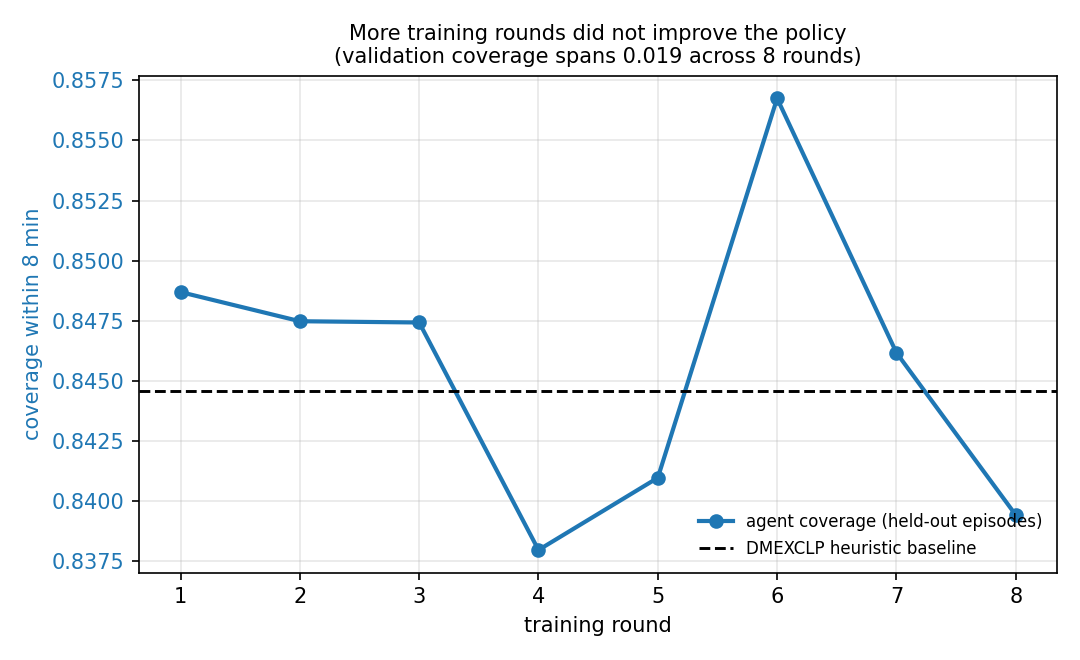
\includegraphics[width=\columnwidth]{../results/figures/learning_curve.png}
\caption{Validation coverage over training rounds, against the heuristic baseline on the
same episodes. Eight rounds produce no upward trend.}
\end{figure}

\begin{figure}[t]
\centering
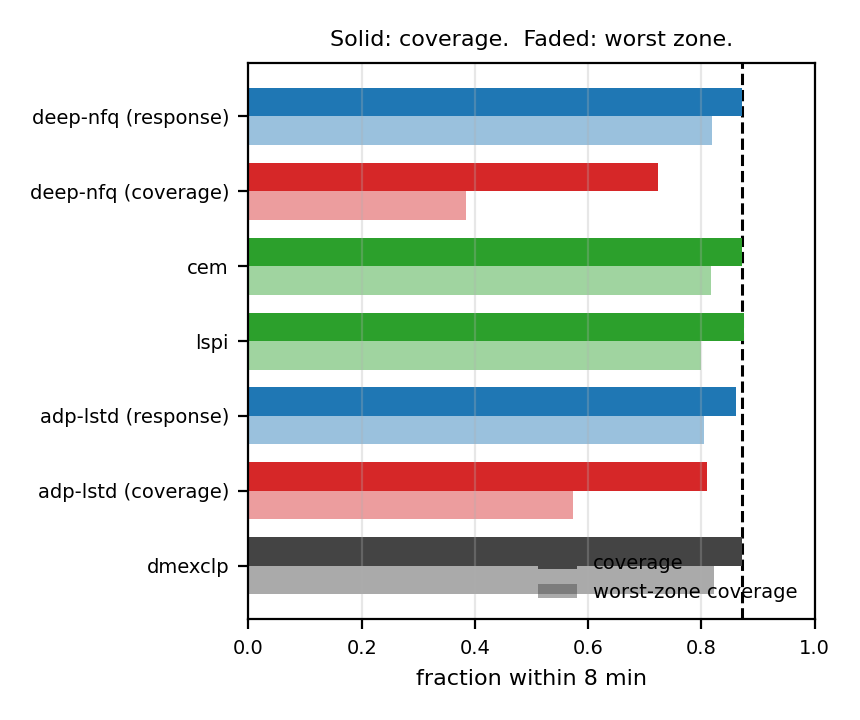
\includegraphics[width=\columnwidth]{../results/figures/phase4_reward_compact.png}
\caption{Reward design dominates model class; the binary reward also collapses worst-zone
coverage.}
\end{figure}

\section{Conclusions}
Four findings, each measured rather than asserted. \textbf{(i)} Reward design dominated
model class: binary versus shaped reward moved coverage by $0.148$, more than any
architectural choice tested. \textbf{(ii)} Value-prediction accuracy is not policy
quality; a control sharing the hypothesis class exactly, but optimising the policy
directly, performed better than the fitted value function. \textbf{(iii)} The learned
policy reaches parity with a strong domain heuristic on the distribution it trained on,
but gives that parity up under demand shift. \textbf{(iv)} Reporting that honestly---with
confidence intervals, disjoint validation and test seeds, and two agreeing significance
tests---is more useful than a tuned victory.

The repository contains the full environment, all agents, the trained network, 66 tests,
and scripts reproducing every figure and table here.

\end{document}
